% Using KOMA Script document style
% Font size setting and
% option to skip empty lines as new paragraphs
\documentclass[10pt,a4paper]{article}
% Packages without Options
\usepackage{
	algorithm,
	alltt,
	algpseudocode,
	amsfonts,
	amssymb,
	appendix,
	array,
	booktabs,
	dirtree,
	enumitem,
	float,
	footnote,
	gensymb,
	geometry,
	graphicx,
	interval,
	karnaugh-map,
	lipsum,
	listings,
	longtable,
	makecell,
	mathtools,
	minted,
  nicematrix,
	parskip,
	pdfpages,
	pgfkeys,
	pgfplots,
	subcaption,
	tabularx,
	tablefootnote,
	textcomp,
	tikz,
    titlecaps,
	venndiagram,
	wrapfig,
	wrapfig,
	xcolor
}



% Packages with Options

\usepackage[framemethod=tikz]{mdframed}
\usepackage[colorlinks,linkcolor=cyan, citecolor=cyan, urlcolor=cyan]{hyperref}
\usepackage[labelfont=bf,textfont=it,labelsep=period]{caption}
\usepackage[RPvoltages]{circuitikz}
\usepackage[english]{babel}
\usepackage[nameinlink,noabbrev]{cleveref}

\definecolor{mintedbackground}{rgb}{0.97,0.97,0.97}

\setminted[cpp]{
bgcolor=mintedbackground,
    linenos=true,
    breaklines=true,}

\setminted[js]{
bgcolor=mintedbackground,
    linenos=true,
    breaklines=true,}

\setminted[python]{
bgcolor=mintedbackground,
    linenos=true,
    breaklines=true,}
    

\linespread{1.5}

% Package: AlgorithmicX
% Sets all comments to be indentend and aligned

\renewcommand{\Comment}[2][.7\linewidth]{%
  \leavevmode\hfill\makebox[#1][l]{//~#2}}


% Package: Interval
% Sets the style of mathematical intervals
\intervalconfig{
soft open fences, separator symbol=,,
}

% Package: Geometry
% Sets the page margins
\geometry{
    a4paper,
    left=32mm,
    right=22mm,
    top=22mm,
    }
	
% Creates a proper caption name for algorithms
\newcommand{\algorithmautorefname}{Algorithm}
\newcommand{\listingautorefname}{Listing}
\algrenewcommand{\algorithmiccomment}[1]{\texttt{// #1} }
% Creates a numbered environment for Theorems
\newtheorem{theorem}{Theorem}

% Redefine the implication arrow to be a simple, thin arrow instead of the default, thick arrow
\renewcommand{\implies}{\rightarrow}

% Create a new command for the set complement to make my logical statements easier to read
\newcommand{\compl}{\overline}

% Creates commands for combinatorics nCr and nPr
\newcommand{\nCr}[2]{\,_{#1}C_{#2}} % nCr
\newcommand{\nPr}[2]{\,_{#1}P_{#2}} % nPr

% Package: tikz
% Loads libraries for drawing automata, 
\usetikzlibrary{automata,positioning,shadows,arrows, shapes.gates.logic.US, calc}

% Creates a command to create a button shape
\newcommand*\keystroke[1]{%
  \tikz[baseline= (key.base)]
    \node[%
      draw,
      fill=white,
      drop shadow={shadow xshift=0.25ex,shadow yshift=-0.25ex,fill=black,opacity=0.75},
      rectangle,
      rounded corners=2pt,
      inner sep=1pt,
      line width=0.5pt,
      font=\scriptsize\sffamily
    ] (key) {#1\strut};
}

% Package: pgfplot
% Sets the global options for PGF Plots
\pgfplotsset{compat=newest}

% Package: tikz
% Flowchart Shapes
\tikzstyle{startstop} = [rectangle, rounded corners, minimum width=3cm, minimum height=1cm,text centered, draw=black, fill=red!30]
\tikzstyle{io} = [trapezium, trapezium left angle=70, trapezium right angle=110, minimum width=3cm, minimum height=1cm, text centered, draw=black, fill=blue!30]
\tikzstyle{process} = [rectangle, minimum width=3cm, minimum height=1cm, text centered, draw=black, fill=orange!30]
\tikzstyle{decision} = [diamond, minimum width=3cm, minimum height=1cm, text centered, draw=black, fill=green!30]
\tikzstyle{arrow} = [thick,->,>=stealth]

% Disable Minted syntax error highlights (red boxes)
\AtBeginEnvironment{minted}{%
  \renewcommand{\fcolorbox}[4][]{#4}}

% Listings Style (non-minted)

\lstdefinestyle{arjuncode}{
    basicstyle=\ttfamily,
    breakatwhitespace=false,         
    breaklines=true,                 
    captionpos=b,                    
    keepspaces=true,                 
    numbers=left,                    
    numbersep=5pt,                  
    showspaces=false,                
    showstringspaces=false,
    showtabs=false,                  
    tabsize=2
}

\lstset{style=arjuncode}

\graphicspath{{images/}}

 %Adjust this based on where your Summary is stored
\title{CM2035: Algorithms \& Data Structures II \\ Summary}
\author{Arjun Muralidharan}
\begin{document}

\maketitle
\newpage
\tableofcontents
\listoffigures
% \listoftables
\listoflistings
% \listofalgorithms

\newpage
\renewcommand{\subsubsectionautorefname}{section\negthinspace}

% WEEKS 1-2

\section{Analysis of Algorithms}
\begin{mdframed}
    \textbf{Learning Outcomes}
    \begin{itemize}[label={\checkmark}]
        \item Determine time and memory consumption of an algorithm described using pseudocode
        \item Determine the growth function of the running time or memory consumption of an algorithm
        \item Use Big-$O$, $\Omega$ and $\Theta$ notations to describe the running time or memory consumption of an algorithm
    \end{itemize}
\end{mdframed}

\subsection{Introduction to Analysis of Algorithms}

We generally assume a generic one-processor, \textbf{\emph{random-access machine (RAM)}}, where instructions are executed one after the other with no concurrent operations.

The RAM model contains instructions commonly found in real computers, including arithmetic, data movement and control, all of which take a constant amount of time. We also assume that that integers generally require around $c \log_{2} n$ bits to store (e.g. the number 8 takes roughly $\log_{2}8=3$ bits to store - it really needs 4 bits) with a constant word size $c \geq 1$ so it does not grow arbitrarily. For example, if the inputs are numbers with 5 digits each, we will require, roughly, at least $5 \log_{2} n$ bits.

Other instructions, such as exponentiation, are not considered constant-time instructions, with the exception of multiplication with $2^k$, which is essentially just shifting a number left by $k$ digits.

Algorithms can be analyzed along the following aspects:

\begin{enumerate}
    \item Correctness
    \item Ease of understanding
    \item Resource consumption
\end{enumerate}

We analyze the resource consumption of algorithms in terms of \textbf{input size} and \textbf{running time}.

\paragraph{Input Size} Generally the number of items in the input, for example the size of an array for sorting. In certain problems it's more appropriate the consider the total number of bits needed to represent the input in memory.

\paragraph{Running Time} The number of primitive operations or ``steps'' executed. We assume that each line $i$ of our pseudocode takes $c_i$ time to execute. The total running time is the sum of the products of \emph{cost per statement} $c_i$ and \emph{executions per statement} $n_i$.

\[    T(n) =  \sum_{i = 1}^{n} c_i n_i  \]

These aspects can be analyzed using either \textbf{empirical measurement} or \textbf{theoretical estimation} --- the latter requires an assumption with regards to the machine model, e.g. the RAM model.

\begin{table}[H]
    \centering
    \begin{tabularx}{\textwidth}{XXX}
        \toprule
                                        & \textbf{Pro}                                    & \textbf{Con}                                               \\ \midrule
        \textbf{Empirical Measurement}  & Real result and no need for manual calculations & Machine-dependent results and higher implementation effort \\
        \textbf{Theoretical Estimation} & Universal results and no implementation effort  & Approximate results and higher manual calculation effort
    \end{tabularx}
    \caption{Advantages and Drawbacks of Analysis Approaches}
\end{table}


When we analyse an algorithm, we can count up space and time units. In \autoref{alg:count1}, the time units taken for execution is 16, counting every memory access, memory write (assignment), logical comparison and control statement once. The space taken is 1, given that only one new variable is created in this algorithm ($a$).

\begin{algorithm}[H]
    \caption{Counting up time and space}
    \label{alg:count1}
    \begin{algorithmic}
        \Function{F1}{\emph{a,b,c}}
        \State{$max = a$} \Comment{1 read, 1 write}
        \If{$b > max$} \Comment{2 read, 1 logical comparison, 1 control statement}
        \State{$max = b$} \Comment{1 read, 1 write}
        \EndIf{}
        \If{$c > max$} \Comment{2 read, 1 logical comparison, 1 control statement}
        \State{$max = c$} \Comment{1 read, 1 write}
        \EndIf{}
        \State{\textbf{return} $max$} \Comment{1 read, 1 control statement}
        \EndFunction{}
    \end{algorithmic}
\end{algorithm}

An algorithm using non-simple operations such as loops is shown in \autoref{alg:count2}. The overall sum of the time units can be calculated as

\[
    1 + (N+1) * 4 + 5N + 3N + 1 = 12N + 6
\]

The algorithm takes only 1 space unit as we are only creating one new variable ($i$).

\begin{algorithm}[H]
    \caption{Counting up time and space}
    \label{alg:count2}
    \begin{algorithmic}
        \Function{F2}{\emph{$A,N,x$}}
        \For{$0 \leq i \leq N $} \Comment{1 write ($i=0$), $(N+1)*$(1 control, 1 logical, 2 read)}
        \If{$ A[i] == x$} \Comment{$N * $ (3 read, 1 logical, 1 control)}
        \State{\textbf{return} $i$} \Comment{does not execute in the worst case}
        \EndIf{}
        \EndFor{} \Comment{$N * $ (1 read, 1 numerical op., 1 write)}
        \State{\textbf{return} -1} \Comment{1 control (no read as we return a fixed number)}
        \EndFunction{}
    \end{algorithmic}
\end{algorithm}

\textbf{Note:} Be mindful of the loop's comparison. If the loop executes until the counter is smaller than some number $N$, the loop will execute it's comparison $N+1$ times and it's afterthought ($i++$) $N$ times, as shown in \autoref{alg:count2}. However, if the loop executes until the counter is \emph{equal} to some number ($i \leq N$), then the loop comparison executes $N+2$ times, and the loop afterthought executes $N+1$ times.

When dealing with \emph{while} loops, first determine how often the condition will be checked, and how often the loop will be executed. This will determine the time units used for running the loop, and then running the loop instructions.

\subsection{Growth of Functions}

Because the RAM model makes simplifying assumptions about a computer, we don't need the precision we get when counting time and space units. Instead, it is sufficient to observe how the running time grows as a function of the input size. Various functions are shown in increasing order of time complexity in \autoref{tab:bigo}. The graphs of various functions is shown in \autoref{fig:bigo}.

\begin{table}[ht]
    \centering
    \begin{tabular}{ll}
        \toprule
        \textbf{Type}   & \textbf{Notation}                                \\ \midrule
        Constant        & \( \mathcal{O}(1) \)                             \\
        Logarithmic     & \(\mathcal{O}(\log(n)) =\mathcal{O}(\log(n^c))\) \\
        Polylogarithmic & \(\mathcal{O}((\log(n))^c) \)                    \\
        Linear          & \(\mathcal{O}(n) \)                              \\
        Quadratic       & \(\mathcal{O}(n^2) \)                            \\
        Polynomial      & \(\mathcal{O}(n^c) \)                            \\
        Exponential     & \(\mathcal{O}(c^n) \)                            \\
        \bottomrule
    \end{tabular}
    \caption{Growth of functions}\label{tab:bigo}
\end{table}

\begin{figure}[H]
    \centering
    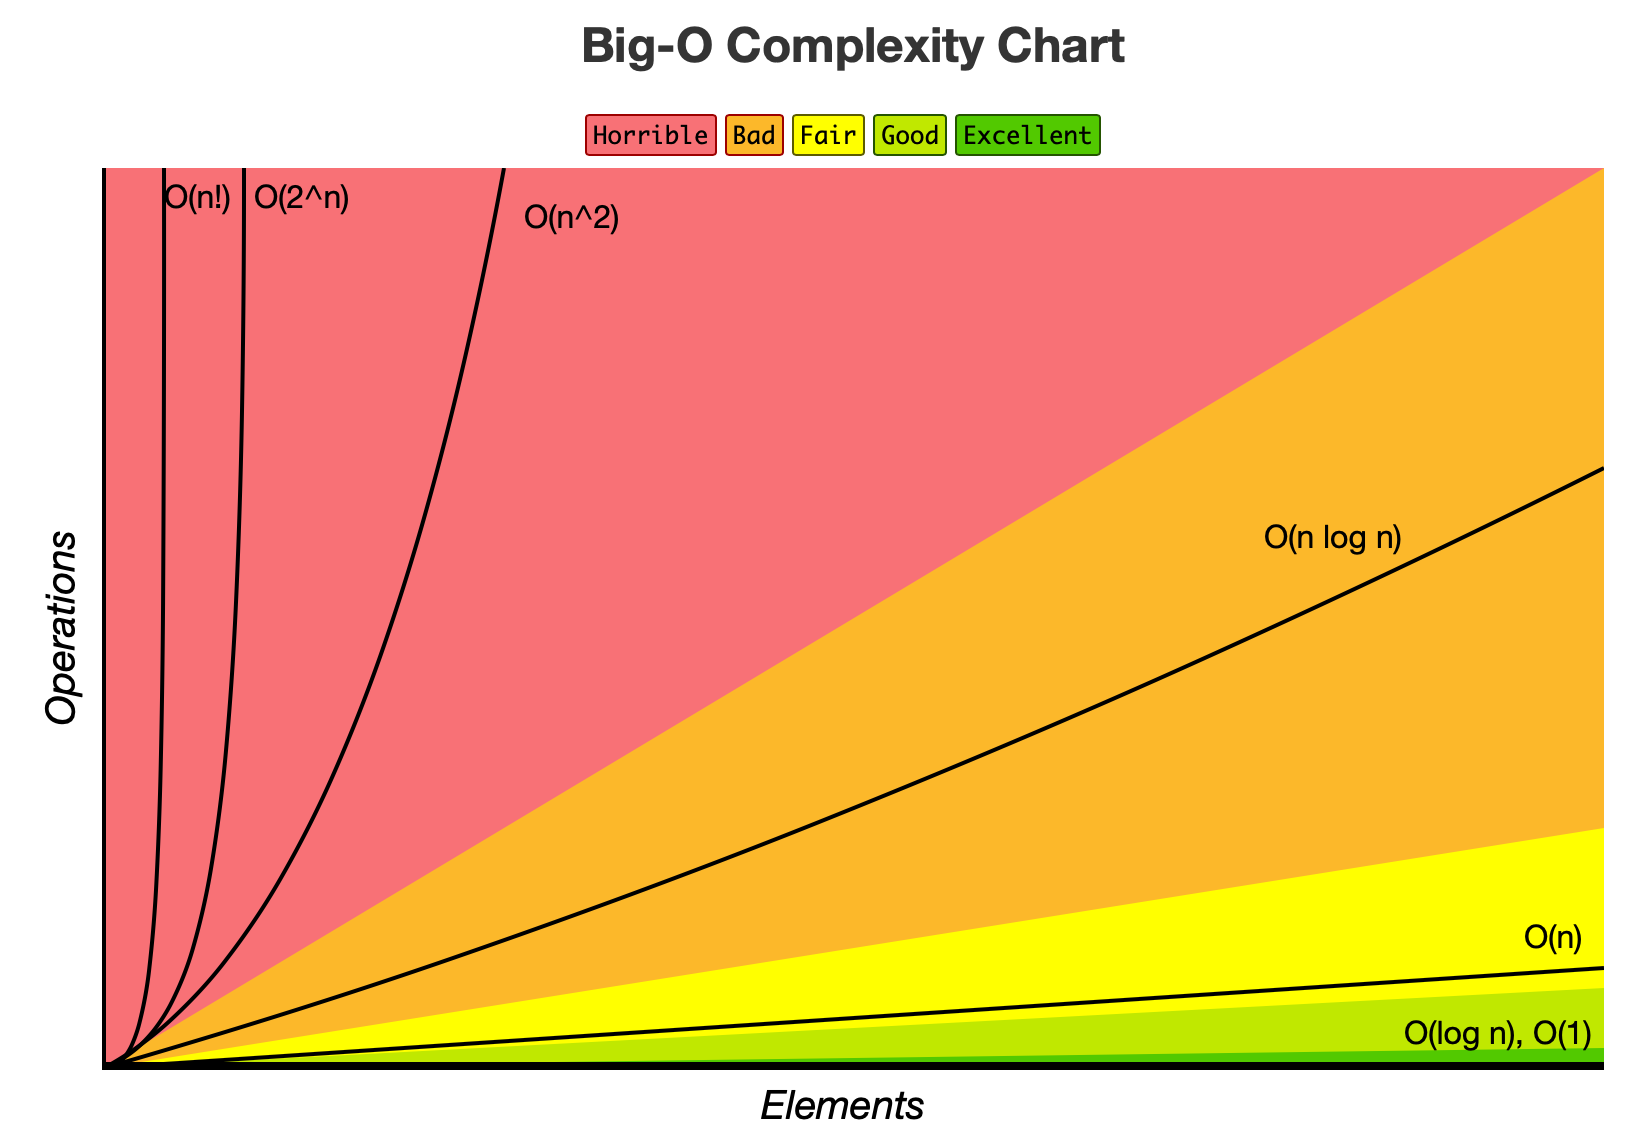
\includegraphics[width=10cm]{bigo.png}
    \caption{Graphs of functions} \label{fig:bigo}
\end{figure}

Investing time in faster algorithms is generally preferable to investing in faster computing infrastructure, because algorithms might run faster on faster algorithms, but they still grow at the same rate relative to the input size. Much greater gains can be made by moving to an algorithm of a different order of growth.

Some algorithms, like a procedure to find the largest element in an array, have identical \emph{best} and \emph{worst} case running times. In other cases, we are interested in the \emph{worst-case} running time, as this gives us an upper bound of the time units taken to execute an algorithm. These cases arise then the \emph{content} of the input data changes the growth function in addition to the input size.

\begin{figure}[H]
    \centering
    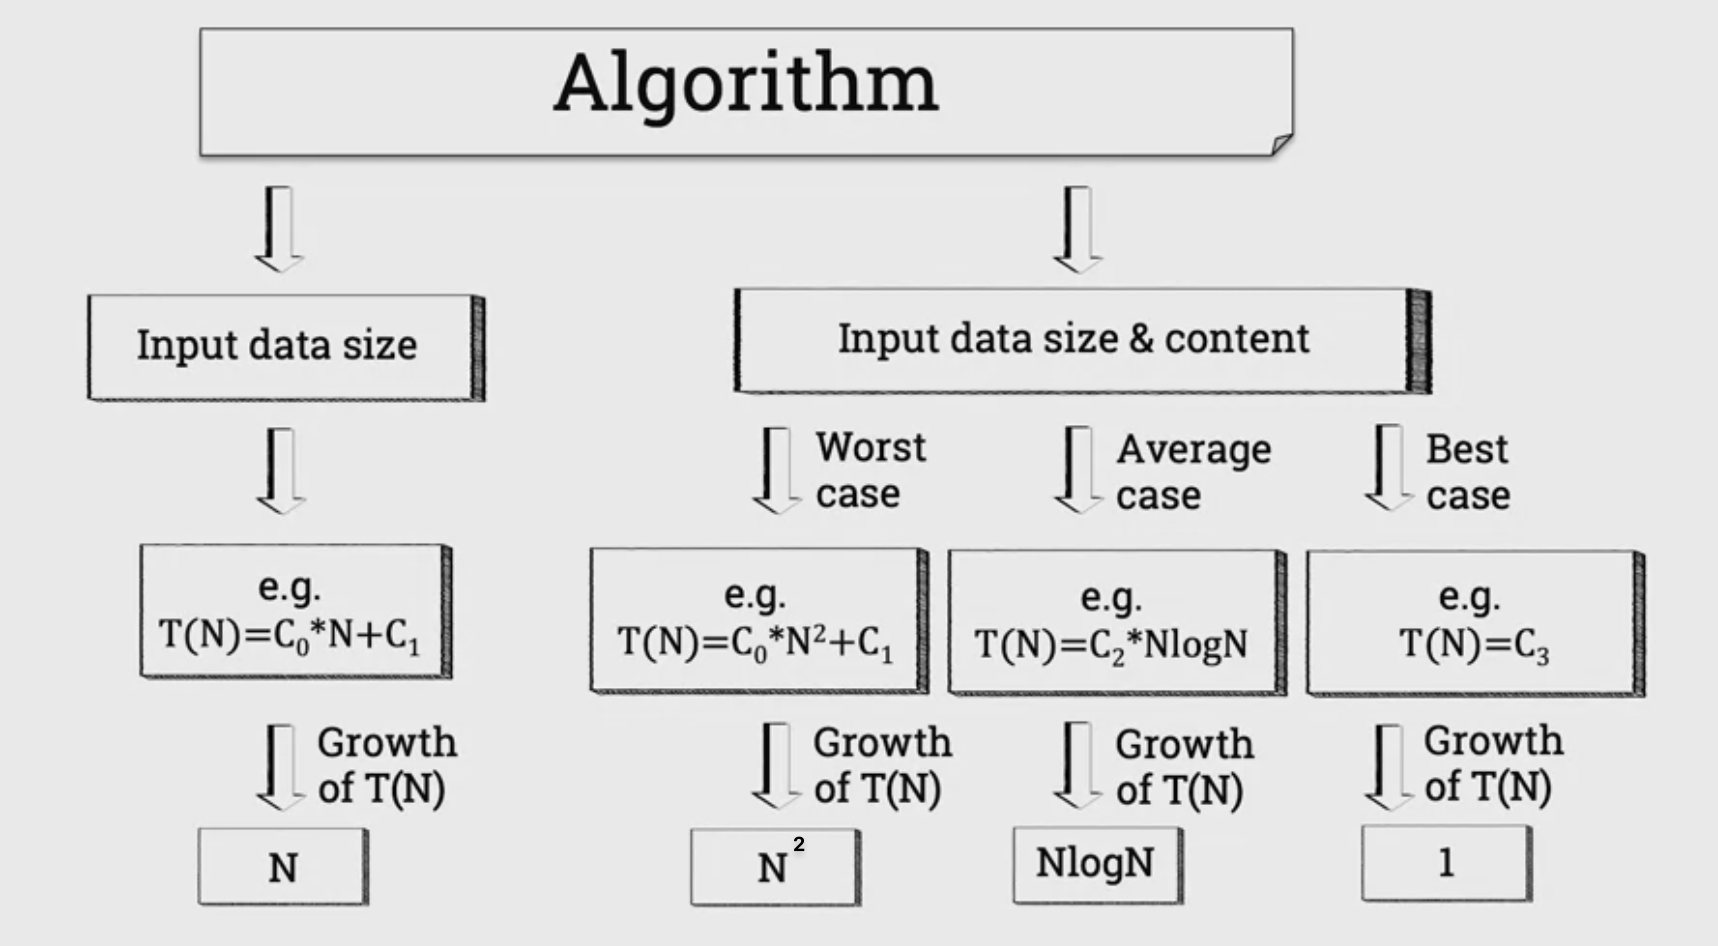
\includegraphics[width=\textwidth]{inputsize.png}
    \caption{Analyzing content in addition to input size}
    \label{fig:inputsize}
\end{figure}

\subsection{Asymptotic Analysis}

Let \( M \) be a RAM machine that halts on all inputs. The \textbf{running time} or \textbf{time complexity} of \( M \) is the function \( f: N \rightarrow N \), where \( f(n) \) is the maximum number of steps that \( M \) uses on any input of length \( n \) . If \( f(n) \) is the running time of \( M \) , we say that \( M \) runs in time \( f(n) \) and that \( M \) is an \( f(n) \) time random access machine. Customarily we use \( n \) to represent the length of the input.

\subsubsection{Big-O Notation}

The \textbf{running time} of an algorithm on a particular input is the number of steps executed. Machine-independently, we define ``time-steps''. The total running time of an algorithm is defined as
\[
    \textrm{time cost per statement} \times \textrm{no. of executions per statement} = \textrm{total running time}
\]

Function growth can be described and compared using \textbf{Big-O Notation}. In \emph{asymptotic analysis}, we can consider only the highest order terms of a function and ignore the constants. For example, given the function \[
    f(n) = 6n^3 + 2n^2 + 20n +45
\]

then the \emph{asymptotic} or \emph{Big-O} notation is given as

\[
    f(n) = \mathcal{O}(n^3)
\]

A table of common functions and their respective Big-O notation is shown in \autoref{tab:bigo} and sorted by growth rate from slowest to fastest.

\begin{table}[ht]
    \centering
    \begin{tabular}{ll}
        \toprule
        \textbf{Type}   & \textbf{Notation}                                \\ \midrule
        Constant        & \( \mathcal{O}(1) \)                             \\
        Logarithmic     & \(\mathcal{O}(\log(n)) =\mathcal{O}(\log(n^c))\) \\
        Polylogarithmic & \(\mathcal{O}((\log(n))^c) \)                    \\
        Linear          & \(\mathcal{O}(n) \)                              \\
        Quadratic       & \(\mathcal{O}(n^2) \)                            \\
        Polynomial      & \(\mathcal{O}(n^c) \)                            \\
        Exponential     & \(\mathcal{O}(c^n) \)                            \\
        \bottomrule
    \end{tabular}
    \caption{Notation in Pseudocode}\label{tab:bigo2}
\end{table}

Formally, this means that any function is asymptotically \emph{upper-bounded} by its respective Big-O class.

Let \( f \) and \( g \) be functions. It holds that

\[
    \exists k \exists n_0 \forall n \{|f(n)| \leq k \cdot g(n) \mid k > 0, n > n_0  \} \implies f(n) \in \mathcal{O}(g(n))
\]
stating that the size of the function \( f(n) \) will eventually be overtaken by the Big-O class \( g(n) \) multiplied by a constant \( k \). It is an upper bound.

Because Big-O classes live inside each other, we always seek to ascertain the \emph{smallest} Big-O class in which a function exists. It states the \textbf{worst-case running time}.

\subsection{Omega Notation}

Omega notation defines the lower bound of a function. It expresses when a function grows at least as fast as \(\Omega(N)\) at large values of \(N\).

Let \( f \) and \( g \) be functions. It holds that

\[
    \exists k \exists n_0 \forall n \{0 \leq k \cdot g(n) \leq |f(n)| \mid k > 0, n > n_0  \} \implies f(n) \in \Omega(g(n))
\]
stating that the size of the function \( f(n) \) will always be larger than \( g(n) \) multiplied by a constant \( k \). It is a lower bound, and states the \textbf{best-case running time}.

\subsection{Theta Notation}

Theta notation defines a function that is both an upper and a lower bound, depending on the constant the function \(g(N)\) is multiplied by.

Let \( f \) and \( g \) be functions. It holds that

\[
    \exists k_1 \exists k_2 \exists n_0 \forall n \{0 \leq k_1 \cdot g(n) \leq |f(n)| \leq k_2 \cdot g(n) \mid k > 0, n > n_0  \} \implies f(n) \in \Theta(g(n))
\]
stating that the size of the function \( f(n) \) will always be exactly between two bounds. It is a statement of the \textbf{average case running time}.


% WEEKS 3-4

\section{Recursive Algorithms}
\begin{mdframed}
    \textbf{Learning Outcomes}
    \begin{itemize}[label={\checkmark}]
        \item Trace and write recursive algorithms
        \item Write the recursive version of an iterative algorithm using pseudocode
        \item Calculate the time complexity of recursive algorithms
    \end{itemize}
\end{mdframed}

\subsection{Structure of Recursive Algorithms}

A recursive algorithm is an algorithm that invokes itself.

\begin{algorithm}[H]
    \caption{Basic structure of a recursive algorithm}
    \label{alg:recursive}
    \begin{algorithmic}
        \Function{hello}{}
        \State{print(``hello'')}
        \State{hello()}
        \EndFunction{}
    \end{algorithmic}
\end{algorithm}

Each call to a recursive function pauses the calling function until the called function completes. The algorithm in \autoref{alg:recursive} never ends, and is an example of \textit{infinite recursion}.

\begin{algorithm}[H]
    \caption{Basic structure of a recursive algorithm}
    \label{alg:recursivefinite}
    \begin{algorithmic}
        \Function{hello}{}
        \If{$n==0$}
        \State{return}
        \EndIf{}
        \State{print(``hello'')}
        \State{hello($n-1$)}
        \EndFunction{}
    \end{algorithmic}
\end{algorithm}

A \textit{finite recursive algorithm} needs to have at least one \textbf{base case}, and a recursive call with an input argument that gets closer to the base case, as shown in \autoref{alg:recursivefinite}.

Recursive solutions are more concise than iterative solutions, however, they are harder to understand and require more memory, as they occupy more space in the call stack.


\subsection{Writing Recursive Algorithms}

\subsubsection{Transforming iterative algorithms to recursive algorithms}

To transform an iterative algorithm into a recursive one, there are three steps.

\begin{enumerate}
    \item \textbf{Initial Value:} Iterative algorithms set the initial value of the iterations by initializing the counter of a loop. Recursive alogrithms do this by setting the input argument to the function.
    \item \textbf{Repetition:} The initial value is checked for a condition. Iterative: In the loop definition; Recursive: As a conditional in the function.
    \item \textbf{Updating the control variable:} Iterative: In the loop afterthought; Recursive: In the recursive call.
\end{enumerate}

\subsection{Analysing Recursive Algorithms}

\subsubsection{Time Complexity of Recursive Algorithms}
The time complexity of an algorithm is the \textit{asymptotic} number of simple operations executed by an algorithm.

The running time \(T(N)\) of a recursive algorithm can be expressed with a \textbf{recurrence equation}, expressed in terms of the running time of the \textit{same algorithm} with \textit{smaller inputs.} For example:

\[
    T(N) = C + T(N-1)
\]

When solving a recurrence relation, there are two steps:

\begin{enumerate}
    \item Find a value of $N$ for which $T(N)$ is known.
    \item Expand the right side of the recurrence relation.
    \item Keep going until you identify the relationship / growth of all coefficients
    \item Replace all coefficients with an expression in terms of  $k$
    \item Replace $k$ with a value so that expressions of $T(N)$ can be replaced by known values (often $C$, $0$ or $1$).
\end{enumerate}

Example where T(1) = C

\begin{align*}
    T(N) & = C_5+T(N-1)           \\
    T(N) & = C_5+(C_5+T(N-1-1))   \\
    T(N) & = C_5+(C_5+T(N-2))     \\
    \vdots                        \\
    T(N) & = k*C_5+T(N-k)         \\
    T(N) & = (N-1)*C_5+T(N-(N-1)) \\
    T(N) & = (N-1)*C_5+T(1)       \\
    T(N) & = (N-1)*C_5+C          \\
    T(N) & = C_5N + C_6
\end{align*}

\subsection{Master Theorem}
A faster way to determine the time complexity of recursive algorithm is to use the Master theorem.

If $a \geq 1$ and $b > 1$ are constants and $f(n)$ is an asymptotically positive function, then  then the time complexity of a recursive relation

\[
    T(n) = a*T(\frac{n}{b}) + f(n)
\]

is given by

\begin{enumerate}
    \item If $f(n) = \mathcal{O}(n^{\log_b a-\epsilon})$, then $T(n) = \Theta(n^{\log_b a})$.
    \item If $f(n) = \Theta(n^{\log_b a})$, then $T(n) = \Theta(n^{\log_b a} * \log n)$.
    \item If $f(n)$ = $\Omega(n^{\log_b a+\epsilon})$, then $T(n) = \Theta(f(n))$.
\end{enumerate}


% WEEKS 5-6

\section{Comparison Sorting Algorithms}
\begin{mdframed}
    \textbf{Learning Outcomes}
    \begin{itemize}[label={\checkmark}]
        \item Identify the different approaches of different comparison sorting algorithms
        \item Implement different comparison sorting algorithms
        \item Calculate the time complexity of different comparison sorting algorithms
    \end{itemize}
\end{mdframed}

\subsection{Comparison and non-comparison sorting algorithms}

The most known comparison sort algorithms are shown in \autoref{tab:comparisonsort}.

\begin{table}[H]
    \centering
    \caption{Comparison Sort Algorithms}
    \label{tab:comparisonsort}
    \begin{tabular}[width=10cm]{lll}
        \hline
                           & \textbf{Worst Case}     & \textbf{Best Case} \\ \hline
        \textbf{Bubble}    & $\mathcal{O}(N^2)$      & $\Omega(N)$        \\
        \textbf{Insertion} & $\mathcal{O}(N^2)$      & $\Omega(N)$        \\
        \textbf{Selection} & $\mathcal{O}(N^2)$      & $\Omega(N^2)$      \\
        \textbf{Quicksort} & $\mathcal{O}(N^2)$      & $\Omega(N \log N)$ \\
        \textbf{Mergesort} & $\mathcal{O}(N \log N)$ & $\Omega(N \log N)$
    \end{tabular}
\end{table}

There are no faster algorithms among comparison sort algorithms than Mergesort. Because they examine every element in the input, they can't be faster than $\mathcal{O}(N \log N)$.

Therefore, we resort to non-comparison sorting algorithms.

\subsection{Bubble Sort}
Bubble sort is popular, but inefficient, sorting algorithm. It works by repeatedly swapping adjacent elements that are out of order.

It starts at the head of a vector, compares the element to the adjacent elements, and swaps the elements if the first element is larger than the second element.

\paragraph{Passes} The Bubble sort algorithm may need multiple passes to sort the entire vector. The maximum number of passes is given by the most difficult vectors to solve - such that are completely in reverse order. In this case, the number of required passes is \( n-1 \) where \( n \) is the number of elements. Therefore, \textbf{the maximum number of passes required} is always \( n-1 \).  

\begin{algorithm}[H]
	\caption{Bubble Sort --- \( \mathcal{O}(n^2) \) }\label{alg:bubble}
	\begin{algorithmic}
		\Function{Bubblesort}{\emph{vector}}
		\State{\( n \leftarrow\) LENGTH[\( vector \)] }
		\For{\( 1 \leq i \leq n-1 \) }
		\State{\( count \leftarrow 0\) }
		\For{\( 1 \leq j \leq n-1 \)}
		\If{\( vector[j+1] < vector[j] \) }
		\State{Swap(\(vector,j,j+1\))}
		\State{\( count \leftarrow count +1 \) }
		\EndIf{}
		\EndFor{}
		\If{\( count = 0 \) }
		\State{\textbf{break} }
		\EndIf{}
		\EndFor{}
		\State{\textbf{return} \emph{vector} }
		\EndFunction{}
	\end{algorithmic}
\end{algorithm}


\subsection{Insertion Sort}
Insertion sort works from the left of a vector, starting with the second element. It compares the element to the element on the left. If it needs to move, the element is moved along to the left as far as needed.

As an algorithm, we can store the current element in a temporary variable, while we ``move'' elements to the right by overwriting the slots to the right and then restoring the original values from the temporary variable.

\begin{algorithm}[H]
	\caption{Insertion Sort --- \( \mathcal{O}(n^2) \) }\label{alg:insert}
	\begin{algorithmic}
		\Function{InsertionSort}{\emph{v}}
		\For{\( 2 \leq \) LENGTH[v]}
		\State{\( key \leftarrow v[j] \) }
		\State{\( i \leftarrow j - 1 \) }
		\While{\( i > 0 \wedge v[i] > key \) }
		\State{\( v[i+1] \leftarrow v[i] \) }
		\State{\( i \leftarrow i-1 \) }
		\EndWhile{}
		\State{\( v[i+1] \leftarrow key \) }
		\EndFor{}
		\EndFunction{}
	\end{algorithmic}
\end{algorithm}

\section{Random-Access Machines, Growth of Functions and Time Complexity}
\begin{mdframed}
	\textbf{Learning Outcomes}
	\begin{itemize}[label={\checkmark}]
		\item Explain the model of random access machines.
		\item Explain asymptotic growth of functions and worst-case time complexity
		\item Describe worst-case time complexity of bubble and insertion sort
	\end{itemize}
	\end{mdframed}


% WEEKS 7-8

\section{Non-comparison sorting algorithms}
\begin{mdframed}
    \textbf{Learning Outcomes}
    \begin{itemize}[label={\checkmark}]
        \item Identify the different approaches of different non-comparison sorting algorithms
        \item Implement different non-comparison sorting algorithms
        \item Calculate the time complexity of different non-comparison sorting algorithms
    \end{itemize}
\end{mdframed}

\subsection{}



% WEEKS 9-10

\section{Hashing}
\begin{mdframed}
    \textbf{Learning Outcomes}
    \begin{itemize}[label={\checkmark}]
        \item Describe the different methods used to search for data
        \item Describe different collision resolution methods
        \item Implement a hash table with linear probing collision resolution
    \end{itemize}
\end{mdframed}

\subsection{}

% WEEKS 11-12 are midterm


% WEEKS 13-14

\section{Linear Data Structures}
\begin{mdframed}
    \textbf{Learning Outcomes}
    \begin{itemize}[label={\checkmark}]
        \item Describe linear data structures and its operations using pseudocode
        \item Understand array and linked list based implementations of stacks and queues
        \item Implement a sorted linked list
    \end{itemize}
\end{mdframed}

\subsection{}


% WEEKS 15-16

\section{Trees}
\begin{mdframed}
    \textbf{Learning Outcomes}
    \begin{itemize}[label={\checkmark}]
        \item Understand how to implement a tree
        \item Describe and trace different types of binary tree traversals using pseudocode
        \item Describe and trace binary search tree operations using pseudocode
    \end{itemize}
\end{mdframed}

\subsection{}


% WEEKS 17-18

\section{Heaps}
\begin{mdframed}
    \textbf{Learning Outcomes}
    \begin{itemize}[label={\checkmark}]
        \item Check heap and shape properties
        \item Describe heap operations using pseudocode
        \item Implement heapsort using a heap
    \end{itemize}
\end{mdframed}

\subsection{}



% WEEKS 19-20

\section{Graphs}
\begin{mdframed}
    \textbf{Learning Outcomes}
    \begin{itemize}[label={\checkmark}]
        \item Use different implementations of graphs (matrix adjacency, list adjacency. Edge list)
        \item Implement Prim’s algorithm to find the minimum spanning tree
        \item Implement Dijkstra’s algorithm to find the shortest path between two nodes
    \end{itemize}
\end{mdframed}

\subsection{}



\end{document}

